\documentclass[tikz]{standalone}
\usepackage{pgfplots}
\pgfplotsset{compat=1.15}
\usepackage{mathrsfs}
\usetikzlibrary{arrows,calc}
\usepackage{tkz-euclide}

\usepackage{fp}
\pagestyle{empty}

\definecolor{AngleClr}{rgb}{0,0.39215686274509803,0}
\definecolor{ShapeClr}{rgb}{0.6,0.2,0}

\begin{document}

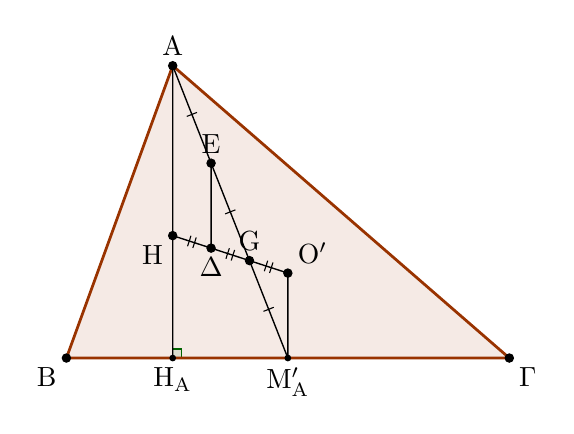
\begin{tikzpicture}[scale=.75]
\tkzSetUpLine[line width=1pt,color=black]
\tkzSetUpPoint[fill=black]

\tkzDefPoints{0/0/B,1.8/4.95/A,7.5/0/C}

\tkzDefTriangleCenter[circum](A,B,C) \tkzGetPoint{O}
\tkzDefTriangleCenter[centroid](A,B,C) \tkzGetPoint{G}
\tkzDefTriangleCenter[ortho](A,B,C) \tkzGetPoint{H}

\tkzDefPointBy[projection = onto B--C](H) \tkzGetPoint{HA}

\tkzDefMidPoint(B,C) \tkzGetPoint{MA}
\tkzDefMidPoint(H,G) \tkzGetPoint{D}
\tkzDefMidPoint(A,G) \tkzGetPoint{E}


\tkzFillPolygon[fill=ShapeClr,fill opacity=0.1](A,B,C)

\tkzMarkRightAngle[line width=0.5pt, size=.15,color=AngleClr,fill=AngleClr,fill opacity=0.1](A,HA,C)

\tkzDrawPolygon[color=ShapeClr](A,B,C)

\tkzDrawSegments[line width=0.5pt,color=black](A,MA A,HA E,D O,H MA,O)

\tkzDrawPoints[size=3](A,B,C,D,E,H,G,O)
\tkzDrawPoints[size=2](HA,MA)
\tkzLabelPoint[above](A){$\rm A$}
\tkzLabelPoint[below left](B){$\rm B$}
\tkzLabelPoint[below right](C){$\rm \Gamma$}
\tkzLabelPoint[below](D){$\rm \Delta$}
\tkzLabelPoint[above](E){$\rm E$}
\tkzLabelPoint[above right](O){$\rm O'$}
\tkzLabelPoint[below left](H){$\rm H$}
\tkzLabelPoint[above](G){$\rm G$}
\tkzLabelPoint[below](MA){$\rm M_A'$}
\tkzLabelPoint[below](HA){$\rm H_A$}

\tkzMarkSegments[mark=|,size=2](A,E E,G G,MA)
\tkzMarkSegments[mark=||,size=2](H,D D,G G,O)

\end{tikzpicture}

\end{document}
